%
% 6.006 problem set 1 solutions template
%


\documentclass[12pt,twoside]{article}

\usepackage{tikz}
\usetikzlibrary{trees}

\usepackage{amsmath}
\usepackage{color}

% Cross-references for handout numbers.

\newcommand{\name}{}

\usepackage{latexsym}
%\usepackage{bbm}
\usepackage{times,url}
\usepackage{clrscode}

\newcommand{\mitst}[1]{\begin{description}
\item[MIT students:] #1
\end{description}}
\newcommand{\smast}[1]{\begin{description}
\item[SMA students:] #1
\end{description}}

\newcommand{\profs}{Professors Erik Demaine, Debayan Gupta, and Ronitt Rubinfeld}
\newcommand{\subj}{6.006}

\newlength{\toppush}
\setlength{\toppush}{2\headheight}
\addtolength{\toppush}{\headsep}

\newcommand{\htitle}[2]{\noindent\vspace*{-\toppush}\newline\parbox{6.5in}
{\textit{Introduction to Algorithms: 6.006}\hfill\name\newline
Massachusetts Institute of Technology \hfill #2\newline
\profs\hfill #1 \vspace*{-.5ex}\newline
\mbox{}\hrulefill\mbox{}}\vspace*{1ex}\mbox{}\newline
\begin{center}{\Large\bf #1}\end{center}}

\newcommand{\handout}[2]{\thispagestyle{empty}
 \markboth{#1}{#1}
 \pagestyle{myheadings}\htitle{#1}{#2}}

\newcommand{\htitlewithouttitle}[2]{\noindent\vspace*{-\toppush}\newline\parbox{6.5in}
{\textit{Introduction to Algorithms}\hfill#2\newline
Massachusetts Institute of Technology \hfill 6.006\newline
%Singapore-MIT Alliance \hfill SMA5503\newline
\profs\hfill Handout #1\vspace*{-.5ex}\newline
\mbox{}\hrulefill\mbox{}}\vspace*{1ex}\mbox{}\newline}

\newcommand{\handoutwithouttitle}[2]{\thispagestyle{empty}
 \markboth{Handout \protect\ref{#1}}{Handout \protect\ref{#1}}
 \pagestyle{myheadings}\htitlewithouttitle{\protect\ref{#1}}{#2}}

\newcommand{\exam}[2]{% parameters: exam name, date
 \thispagestyle{empty}
 \markboth{\subj\ #1\hspace{1in}Name\hrulefill\ \ }%
          {\subj\ #1\hspace{1in}Name\hrulefill\ \ }
 \pagestyle{myheadings}\examtitle{#1}{#2}
 \renewcommand{\theproblem}{Problem \arabic{problemnum}}
}
\newcommand{\examsolutions}[3]{% parameters: handout, exam name, date
 \thispagestyle{empty}
 \markboth{Handout \protect\ref{#1}: #2}{Handout \protect\ref{#1}: #2}
% \pagestyle{myheadings}\htitle{\protect\ref{#1}}{#2}{#3}
 \pagestyle{myheadings}\examsolutionstitle{\protect\ref{#1}} {#2}{#3}
 \renewcommand{\theproblem}{Problem \arabic{problemnum}}
}
\newcommand{\examsolutionstitle}[3]{\noindent\vspace*{-\toppush}\newline\parbox{6.5in}
{\textit{Introduction to Algorithms}\hfill#3\newline
Massachusetts Institute of Technology \hfill 6.006\newline
%Singapore-MIT Alliance \hfill SMA5503\newline
\profs\hfill Handout #1\vspace*{-.5ex}\newline
\mbox{}\hrulefill\mbox{}}\vspace*{1ex}\mbox{}\newline
\begin{center}{\Large\bf #2}\end{center}}

\newcommand{\takehomeexam}[2]{% parameters: exam name, date
 \thispagestyle{empty}
 \markboth{\subj\ #1\hfill}{\subj\ #1\hfill}
 \pagestyle{myheadings}\examtitle{#1}{#2}
 \renewcommand{\theproblem}{Problem \arabic{problemnum}}
}

\makeatletter
\newcommand{\exambooklet}[2]{% parameters: exam name, date
 \thispagestyle{empty}
 \markboth{\subj\ #1}{\subj\ #1}
 \pagestyle{myheadings}\examtitle{#1}{#2}
 \renewcommand{\theproblem}{Problem \arabic{problemnum}}
 \renewcommand{\problem}{\newpage
 \item \let\@currentlabel=\theproblem
 \markboth{\subj\ #1, \theproblem}{\subj\ #1, \theproblem}}
}
\makeatother


\newcommand{\examtitle}[2]{\noindent\vspace*{-\toppush}\newline\parbox{6.5in}
{\textit{Introduction to Algorithms}\hfill#2\newline
Massachusetts Institute of Technology \hfill 6.006 Spring 2014\newline
%Singapore-MIT Alliance \hfill SMA5503\newline
\profs\hfill #1\vspace*{-.5ex}\newline
\mbox{}\hrulefill\mbox{}}\vspace*{1ex}\mbox{}\newline
\begin{center}{\Large\bf #1}\end{center}}

\newcommand{\grader}[1]{\hspace{1cm}\textsf{\textbf{#1}}\hspace{1cm}}

\newcommand{\points}[1]{[#1 points]\ }
\newcommand{\parts}[1]
{
  \ifnum#1=1
  (1 part)
  \else
  (#1 parts)
  \fi
  \
}

\newcommand{\bparts}{\begin{problemparts}}
\newcommand{\eparts}{\end{problemparts}}
\newcommand{\ppart}{\problempart}

%\newcommand{\lg} {lg\ }

\setlength{\oddsidemargin}{0pt}
\setlength{\evensidemargin}{0pt}
\setlength{\textwidth}{6.5in}
\setlength{\topmargin}{0in}
\setlength{\textheight}{8.5in}


\newcommand{\Spawn}{{\bf spawn} }
\newcommand{\Sync}{{\bf sync}}

%\renewcommand{\cases}[1]{\left\{ \begin{array}{ll}#1\end{array}\right.}
\newcommand{\cif}[1]{\mbox{if $#1$}}
\newcommand{\cwhen}[1]{\mbox{when $#1$}}

\newcounter{problemnum}
\newcommand{\theproblem}{Problem \theproblemsetnum-\arabic{problemnum}}
\newenvironment{problems}{
        \begin{list}{{\bf \theproblem. \hspace*{0.5em}}}
        {\setlength{\leftmargin}{0em}
         \setlength{\rightmargin}{0em}
         \setlength{\labelwidth}{0em}
         \setlength{\labelsep}{0em}
         \usecounter{problemnum}}}{\end{list}}
\makeatletter
\newcommand{\problem}[1][{}]{\item \let\@currentlabel=\theproblem \textbf{#1}}
\makeatother

\newcounter{problempartnum}[problemnum]
\newenvironment{problemparts}{
        \begin{list}{{\bf (\alph{problempartnum})}}
        {\setlength{\leftmargin}{2.5em}
         \setlength{\rightmargin}{2.5em}
         \setlength{\labelsep}{0.5em}}}{\end{list}}
\newcommand{\problempart}{\addtocounter{problempartnum}{1}\item}

\newenvironment{truefalseproblemparts}{
        \begin{list}{{\bf (\alph{problempartnum})\ \ \ T\ \ F\hfil}}
        {\setlength{\leftmargin}{4.5em}
         \setlength{\rightmargin}{2.5em}
         \setlength{\labelsep}{0.5em}
         \setlength{\labelwidth}{4.5em}}}{\end{list}}

\newcounter{exercisenum}
\newcommand{\theexercise}{Exercise \theproblemsetnum-\arabic{exercisenum}}
\newenvironment{exercises}{
        \begin{list}{{\bf \theexercise. \hspace*{0.5em}}}
        {\setlength{\leftmargin}{0em}
         \setlength{\rightmargin}{0em}
         \setlength{\labelwidth}{0em}
         \setlength{\labelsep}{0em}
        \usecounter{exercisenum}}}{\end{list}}
\makeatletter
\newcommand{\exercise}{\item \let\@currentlabel=\theexercise}
\makeatother

\newcounter{exercisepartnum}[exercisenum]
%\newcommand{\problem}[1]{\medskip\mbox{}\newline\noindent{\bf Problem #1.}\hspace*{1em}}
%\newcommand{\exercise}[1]{\medskip\mbox{}\newline\noindent{\bf Exercise #1.}\hspace*{1em}}

\newenvironment{exerciseparts}{
        \begin{list}{{\bf (\alph{exercisepartnum})}}
        {\setlength{\leftmargin}{2.5em}
         \setlength{\rightmargin}{2.5em}
         \setlength{\labelsep}{0.5em}}}{\end{list}}
\newcommand{\exercisepart}{\addtocounter{exercisepartnum}{1}\item}


% Macros to make captions print with small type and 'Figure xx' in bold.
\makeatletter
\def\fnum@figure{{\bf Figure \thefigure}}
\def\fnum@table{{\bf Table \thetable}}
\let\@mycaption\caption
%\long\def\@mycaption#1[#2]#3{\addcontentsline{\csname
%  ext@#1\endcsname}{#1}{\protect\numberline{\csname
%  the#1\endcsname}{\ignorespaces #2}}\par
%  \begingroup
%    \@parboxrestore
%    \small
%    \@makecaption{\csname fnum@#1\endcsname}{\ignorespaces #3}\par
%  \endgroup}
%\def\mycaption{\refstepcounter\@captype \@dblarg{\@mycaption\@captype}}
%\makeatother
\let\mycaption\caption
%\newcommand{\figcaption}[1]{\mycaption[]{#1}}

\newcounter{totalcaptions}
\newcounter{totalart}

\newcommand{\figcaption}[1]{\addtocounter{totalcaptions}{1}\caption[]{#1}}

% \psfigures determines what to do for figures:
%       0 means just leave vertical space
%       1 means put a vertical rule and the figure name
%       2 means insert the PostScript version of the figure
%       3 means put the figure name flush left or right
\newcommand{\psfigures}{0}
\newcommand{\spacefigures}{\renewcommand{\psfigures}{0}}
\newcommand{\rulefigures}{\renewcommand{\psfigures}{1}}
\newcommand{\macfigures}{\renewcommand{\psfigures}{2}}
\newcommand{\namefigures}{\renewcommand{\psfigures}{3}}

\newcommand{\figpart}[1]{{\bf (#1)}\nolinebreak[2]\relax}
\newcommand{\figparts}[2]{{\bf (#1)--(#2)}\nolinebreak[2]\relax}


\macfigures     % STATE

% When calling \figspace, make sure to leave a blank line afterward!!
% \widefigspace is for figures that are more than 28pc wide.
\newlength{\halffigspace} \newlength{\wholefigspace}
\newlength{\figruleheight} \newlength{\figgap}
\newcommand{\setfiglengths}{\ifnum\psfigures=1\setlength{\figruleheight}{\hruleheight}\setlength{\figgap}{1em}\else\setlength{\figruleheight}{0pt}\setlength{\figgap}{0em}\fi}
\newcommand{\figspace}[2]{\ifnum\psfigures=0\leavefigspace{#1}\else%
\setfiglengths%
\setlength{\wholefigspace}{#1}\setlength{\halffigspace}{.5\wholefigspace}%
\rule[-\halffigspace]{\figruleheight}{\wholefigspace}\hspace{\figgap}#2\fi}
\newlength{\widefigspacewidth}
% Make \widefigspace put the figure flush right on the text page.
\newcommand{\widefigspace}[2]{
\ifnum\psfigures=0\leavefigspace{#1}\else%
\setfiglengths%
\setlength{\widefigspacewidth}{28pc}%
\addtolength{\widefigspacewidth}{-\figruleheight}%
\setlength{\wholefigspace}{#1}\setlength{\halffigspace}{.5\wholefigspace}%
\makebox[\widefigspacewidth][r]{#2\hspace{\figgap}}\rule[-\halffigspace]{\figruleheight}{\wholefigspace}\fi}
\newcommand{\leavefigspace}[1]{\setlength{\wholefigspace}{#1}\setlength{\halffigspace}{.5\wholefigspace}\rule[-\halffigspace]{0em}{\wholefigspace}}

% Commands for including figures with macpsfig.
% To use these commands, documentstyle ``macpsfig'' must be specified.
\newlength{\macfigfill}
\makeatother
\newlength{\bbx}
\newlength{\bby}
\newcommand{\macfigure}[5]{\addtocounter{totalart}{1}
\ifnum\psfigures=2%
\setlength{\bbx}{#2}\addtolength{\bbx}{#4}%
\setlength{\bby}{#3}\addtolength{\bby}{#5}%
\begin{flushleft}
\ifdim#4>28pc\setlength{\macfigfill}{#4}\addtolength{\macfigfill}{-28pc}\hspace*{-\macfigfill}\fi%
\mbox{\psfig{figure=./#1.ps,%
bbllx=#2,bblly=#3,bburx=\bbx,bbury=\bby}}
\end{flushleft}%
\else\ifdim#4>28pc\widefigspace{#5}{#1}\else\figspace{#5}{#1}\fi\fi}
\makeatletter

\newlength{\savearraycolsep}
\newcommand{\narrowarray}[1]{\setlength{\savearraycolsep}{\arraycolsep}\setlength{\arraycolsep}{#1\arraycolsep}}
\newcommand{\normalarray}{\setlength{\arraycolsep}{\savearraycolsep}}

\newcommand{\hint}{{\em Hint:\ }}

% Macros from /th/u/clr/mac.tex

\newcommand{\set}[1]{\left\{ #1 \right\}}
\newcommand{\abs}[1]{\left| #1\right|}
\newcommand{\card}[1]{\left| #1\right|}
\newcommand{\floor}[1]{\left\lfloor #1 \right\rfloor}
\newcommand{\ceil}[1]{\left\lceil #1 \right\rceil}
\newcommand{\ang}[1]{\ifmmode{\left\langle #1 \right\rangle}
   \else{$\left\langle${#1}$\right\rangle$}\fi}
        % the \if allows use outside mathmode,
        % but will swallow following space there!
\newcommand{\paren}[1]{\left( #1 \right)}
\newcommand{\bracket}[1]{\left[ #1 \right]}
\newcommand{\prob}[1]{\Pr\left\{ #1 \right\}}
\newcommand{\Var}{\mathop{\rm Var}\nolimits}
\newcommand{\expect}[1]{{\rm E}\left[ #1 \right]}
\newcommand{\expectsq}[1]{{\rm E}^2\left[ #1 \right]}
\newcommand{\variance}[1]{{\rm Var}\left[ #1 \right]}
\renewcommand{\choose}[2]{{{#1}\atopwithdelims(){#2}}}
\def\pmod#1{\allowbreak\mkern12mu({\rm mod}\,\,#1)}
\newcommand{\matx}[2]{\left(\begin{array}{*{#1}{c}}#2\end{array}\right)}
\newcommand{\Adj}{\mathop{\rm Adj}\nolimits}

\newtheorem{theorem}{Theorem}
\newtheorem{lemma}[theorem]{Lemma}
\newtheorem{corollary}[theorem]{Corollary}
\newtheorem{claim}[theorem]{Claim}
\newtheorem{xample}{Example}
\newtheorem{definition}{Definition}
\newenvironment{example}{\begin{xample}\rm}{\end{xample}}
\newcommand{\proof}{\noindent{\em Proof.}\hspace{1em}}
\def\squarebox#1{\hbox to #1{\hfill\vbox to #1{\vfill}}}
\newcommand{\qedbox}{\vbox{\hrule\hbox{\vrule\squarebox{.667em}\vrule}\hrule}}
\newcommand{\qed}{\nopagebreak\mbox{}\hfill\qedbox\smallskip}
\newcommand{\eqnref}[1]{(\protect\ref{#1})}

%%\newcommand{\twodots}{\mathinner{\ldotp\ldotp}}
\newcommand{\transpose}{^{\mbox{\scriptsize \sf T}}}
\newcommand{\amortized}[1]{\widehat{#1}}

\newcommand{\punt}[1]{}

%%% command for putting definitions into boldface
% New style for defined terms, as of 2/23/88, redefined by THC.
\newcommand{\defn}[1]{{\boldmath\textit{\textbf{#1}}}}
\newcommand{\defi}[1]{{\textit{\textbf{#1\/}}}}

%\newcommand{\red}{\leq_{\rm P}}
\newcommand{\lang}[1]{%
\ifmmode\mathord{\mathcode`-="702D\rm#1\mathcode`\-="2200}\else{\rm#1}\fi}

%\newcommand{\ckt}[1]{\ifmmode\mathord{\mathcode`-="702D\sc #1\mathcode`\-="2200}\else$\mathord{\mathcode`-="702D\sc #1\mathcode`\-="2200}$\fi}
\newcommand{\ckt}[1]{\ifmmode \sc #1\else$\sc #1$\fi}

%% Margin notes - use \notesfalse to turn off notes.
\setlength{\marginparwidth}{0.6in}
\reversemarginpar
\newif\ifnotes
\notestrue
\newcommand{\longnote}[1]{
  \ifnotes
    {\medskip\noindent Note: \marginpar[\hfill$\Longrightarrow$]
      {$\Longleftarrow$}{#1}\medskip}
  \fi}
\newcommand{\note}[1]{
  \ifnotes
    {\marginpar{\tiny \raggedright{#1}}}
  \fi}


\newcommand{\reals}{\mathbbm{R}}
\newcommand{\integers}{\mathbbm{Z}}
\newcommand{\naturals}{\mathbbm{N}}
\newcommand{\rationals}{\mathbbm{Q}}
\newcommand{\complex}{\mathbbm{C}}

\newcommand{\oldreals}{{\bf R}}
\newcommand{\oldintegers}{{\bf Z}}
\newcommand{\oldnaturals}{{\bf N}}
\newcommand{\oldrationals}{{\bf Q}}
\newcommand{\oldcomplex}{{\bf C}}

\newcommand{\w}{\omega}                 %% for fft chapter

\newenvironment{closeitemize}{\begin{list}
{$\bullet$}
{\setlength{\itemsep}{-0.2\baselineskip}
\setlength{\topsep}{0.2\baselineskip}
\setlength{\parskip}{0pt}}}
{\end{list}}

% These are necessary within a {problems} environment in order to restore
% the default separation between bullets and items.
\newenvironment{normalitemize}{\setlength{\labelsep}{0.5em}\begin{itemize}}
                              {\end{itemize}}
\newenvironment{normalenumerate}{\setlength{\labelsep}{0.5em}\begin{enumerate}}
                                {\end{enumerate}}

%\def\eqref#1{Equation~(\ref{eq:#1})}
%\newcommand{\eqref}[1]{Equation (\ref{eq:#1})}
\newcommand{\eqreftwo}[2]{Equations (\ref{eq:#1}) and~(\ref{eq:#2})}
\newcommand{\ineqref}[1]{Inequality~(\ref{ineq:#1})}
\newcommand{\ineqreftwo}[2]{Inequalities (\ref{ineq:#1}) and~(\ref{ineq:#2})}

\newcommand{\figref}[1]{Figure~\ref{fig:#1}}
\newcommand{\figreftwo}[2]{Figures \ref{fig:#1} and~\ref{fig:#2}}

\newcommand{\liref}[1]{line~\ref{li:#1}}
\newcommand{\Liref}[1]{Line~\ref{li:#1}}
\newcommand{\lirefs}[2]{lines \ref{li:#1}--\ref{li:#2}}
\newcommand{\Lirefs}[2]{Lines \ref{li:#1}--\ref{li:#2}}
\newcommand{\lireftwo}[2]{lines \ref{li:#1} and~\ref{li:#2}}
\newcommand{\lirefthree}[3]{lines \ref{li:#1}, \ref{li:#2}, and~\ref{li:#3}}

\newcommand{\lemlabel}[1]{\label{lem:#1}}
\newcommand{\lemref}[1]{Lemma~\ref{lem:#1}}

\newcommand{\exref}[1]{Exercise~\ref{ex:#1}}

\newcommand{\handref}[1]{Handout~\ref{#1}}

\newcommand{\defref}[1]{Definition~\ref{def:#1}}

% (1997.8.16: Victor Luchangco)
% Modified \hlabel to only get date and to use handouts counter for number.
%   New \handout and \handoutwithouttitle commands in newmac.tex use this.
%   The date is referenced by <label>-date.
%   (Retained old definition as \hlabelold.)
%   Defined \hforcelabel to use an argument instead of the handouts counter.

\newcounter{handouts}
\setcounter{handouts}{0}

\newcommand{\hlabel}[2]{%
\stepcounter{handouts}
{\edef\next{\write\@auxout{\string\newlabel{#1}{{\arabic{handouts}}{0}}}}\next}
\write\@auxout{\string\newlabel{#1-date}{{#2}{0}}}
}

\newcommand{\hforcelabel}[3]{%          Does not step handouts counter.
\write\@auxout{\string\newlabel{#1}{{#2}{0}}}
\write\@auxout{\string\newlabel{#1-date}{{#3}{0}}}}


% less ugly underscore
% --juang, 2008 oct 05
\renewcommand{\_}{\vrule height 0 pt depth 0.4 pt width 0.5 em \,}


\setlength{\oddsidemargin}{0pt}
\setlength{\evensidemargin}{0pt}
\setlength{\textwidth}{6.5in}
\setlength{\topmargin}{0in}
\setlength{\textheight}{8.5in}

\newcommand{\theproblemsetnum}{1}
\newcommand{\releasedate}{Tuesday, September 13}
\newcommand{\partaduedate}{Tuesday, September 27}
\newcommand{\tabUnit}{3ex}
\newcommand{\myname}{Milo H. Knowles}

%define collaborators here
\newcommand{\collabs}{Gillian Belton, Magnus Johnson, Kacie Bawiec, Wala'a Alkhanaizi}

\newcommand{\tabT}{\hspace*{\tabUnit}}

\title{6.006 Problem Set 1}

%everything after the begin command is in the document
\begin{document}

\handout{Problem Set \theproblemsetnum}{September 13, 2016}

\textbf{All parts are due {\bf \partaduedate} at {\bf 11:59PM}}.

\setlength{\parindent}{0pt}

\medskip

\hrulefill

\medskip

{\bf Name:} \myname

\medskip

{\bf Collaborators:} \collabs

\medskip

\hrulefill

%%%%%%%%%%%%%%%%%%%%%%%%%%%%%%%%%%%%%%%%%%%%%%%%%%%%%
% See below for common and useful latex constructs. %
%%%%%%%%%%%%%%%%%%%%%%%%%%%%%%%%%%%%%%%%%%%%%%%%%%%%%

% Some useful commands:
%$f(x) = \Theta(x)$
%$T(x, y) \leq \log(x) + 2^y + \binom{2n}{n}$
% {\tt code\_function}


% You can create unnumbered lists as follows:
%\begin{itemize}
%    \item First item in a list 
%        \begin{itemize}
%            \item First item in a list 
%                \begin{itemize}
%                    \item First item in a list 
%                    \item Second item in a list 
%                \end{itemize}
%            \item Second item in a list 
%        \end{itemize}
%    \item Second item in a list 
%\end{itemize}

% You can create numbered lists as follows:
%\begin{enumerate}
%    \item First item in a list 
%    \item Second item in a list 
%    \item Third item in a list
%\end{enumerate}

% You can write aligned equations as follows:
%\begin{align} 
%    \begin{split}
%        (x+y)^3 &= (x+y)^2(x+y) \\
%                &= (x^2+2xy+y^2)(x+y) \\
%                &= (x^3+2x^2y+xy^2) + (x^2y+2xy^2+y^3) \\
%                &= x^3+3x^2y+3xy^2+y^3
%    \end{split}                                 
%\end{align}

% You can create grids/matrices as follows:
%\begin{align}
%    A = 
%    \begin{bmatrix}
%        A_{11} & A_{21} \\
%        A_{21} & A_{22}
%    \end{bmatrix}
%\end{align}

\begin{problems}

%star after section means that the section is not NUMBERED
\section*{Part A}

\problem  % Problem 1

\begin{problemparts}
\problempart In order of increasing growth: $$[(log_2n^2)^2, n, nlogn,  n^2, 2^n ]$$
First,
$$(logn^2)^2 = 4(logn)^2$$ which grows more slowly than $n$ because generally the logarithm of a number is less than the number itself. This also explains why $nlogn$ is before $n^2$. An expression with a growing variable in the exponent will be bigger than an expression with a constant exponent, so $O(2^n)$ is the largest.

\problempart In order of increasing growth: $$[f_1, f_6, f_3, f_5, f_2, f_4]$$
First, some simplifications:
$$f_1 = log((logn)^3) = 3log(logn)$$
$$f_5 = log(3(n^{n^3})) = n^3log(3n)$$
$f_1$ has the smallest order of growth because it is a log of a log. $f_6$ is the next smallest because it has a constant exponent. $f_3$ is raised to the power $logn$ which grows more slowly than the $n^3$ term of  $f_5$. $f_2$ has an exponent that grows with $n$, but $f_4$ is biggest because it has two layers of exponents, one of which is constant, and one of which grows with n.

\problempart In order of increasing growth: $$[f_5, f_1, f_2, f_4, f_3]$$

If we realize that $f_1 = 4^{3n} = 2^{6n}$, then the exponents can be easily compared. Ranking the exponents from smallest to largest will give the correct order for the functions in this group. $$ 5n < 6n < n^4 < 3^n < 3^{n+1} $$
\end{problemparts}



\problem  % Problem 2

\begin{problemparts}

\problempart Solving Recurrences
\begin{enumerate}
	\item $T(n) = 8T(\frac{n}{3})+ n^2 = O(n^2)$
	\item $T(n) = 10T(\frac{n}{3})+ n^2 = O(n^{log_3 10})$
	\item $T(n) = 2T(\frac{n}{2})+ n$ \\
	Using the Master Theorem, $T(n)=O(n log n)$ \\
	Using the recursion tree method: \\
	
	
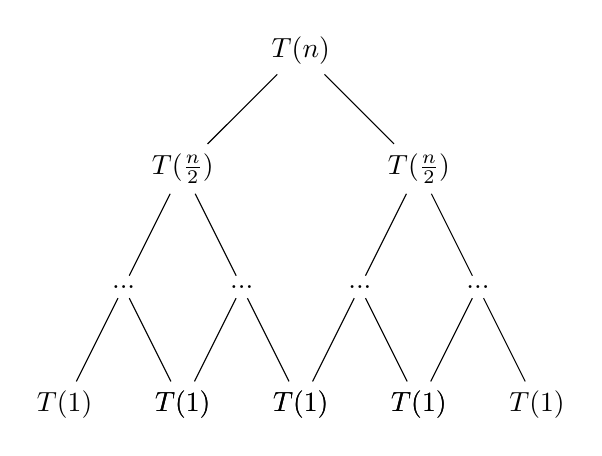
\begin{tikzpicture}[level distance=1.5cm,
  level 1/.style={sibling distance=3cm},
  level 2/.style={sibling distance=1.5cm}]
  \node {$T(n)$}
     child {node {$T(\frac{n}{2})$}
     child {node {$...$}   
     child {node {$T(1)$}}
     child {node {$T(1)$}}
    }
      child {node {$...$}
      child {node {$T(1)$}}
      child {node {$T(1)$}}}
    }
     child {node {$T(\frac{n}{2})$}
     child {node {$...$}
     child {node {$T(1)$}}
     child {node {$T(1)$}}}
     child {node {$...$}
     child {node {$T(1)$}}
     child {node {$T(1)$}}
     } 
     };
\end{tikzpicture} \\
\bigskip
	
	\vspace{5mm}
	
	\item $T(n) = T(\frac{n}{2})+ O(n)$ \\
	Expanding the recurrence: \\
	$T(n) = T(\frac{n}{2}) + O(n)$ \\
	$T(n) = T(\frac{n}{2}) + cn $\\
	$T(n) = T(\frac{n}{4}) + c\frac{n}{2} cn$ \\
	$T(n) = T(\frac{n}{8}) + c\frac{n}{4} + c\frac{n}{2} + cn $\\
	$...$ \\
	$T(n) = T(1) + cn(1 + \frac{1}{2} + \frac{1}{4} + \frac{1}{8} + ... + \frac{1}{2^i})$ \\
	This sum has a finite value, so $T(n) = O(n)$.

\end{enumerate}


\problempart Part b % Problem 2b
\end{problemparts}

\problem  % Problem 3

\begin{problemparts}
\problempart Part a % Problem 3a
\problempart Part b % Problem 3b
\end{problemparts}

\section*{Part B}

\problem
\begin{problemparts}
\problempart \emph{Submit your implementation on alg.csail.mit.edu}
\problempart \emph{Submit your implementation on alg.csail.mit.edu}
\problempart \emph{Submit your implementation on alg.csail.mit.edu}
\problempart Part d % Problem 4d

Below is a list of the constants used in runtime analysis for parts (b) and (c):
\begin{itemize}
	\item $n$, the total number of articles
	\item $m$, the total number of words in each article (assumed to be the same for every article)
	\item $k$, the number of relevant articles to return
	\item $q$, the number of distinct terms in the query (for part (c))
	\item $w$, the number of unique words in the corpus (no repeats)
	\item $l$, the total number of words (with repeats) in the query (for part (c))
\end{itemize}

%make a list of the steps in part(b) with their runtime expressions

%%% STORE NEEDED VARIABLES HERE %%%
\newcommand{\functionb}{get-relevant-articles-tf-idf}
\newcommand{\functionc}{search}

% use \vspace to add vertical space!
\vspace{5mm}

% text for analysis of part (b)
The implementation of {\bf \functionb} from {\bf part(b)} is outlined below:
\begin{enumerate}
	\item For each article, build a term-frequency dictionary. This takes $\theta(nm)$ time, because the code iterates over exactly $n$ articles, and $m$ words in each article.
	\item Next, the function builds a document-frequency dictionary, storing each word in the corpus as a key, and the number of articles that contain that word as a value. This takes $\theta(nm)$ time, because the code iterates over $n$ articles, and $m$ words in each article.
	\item For each {\textit unique} term in the corpus, the inverse-document-frequency is computed and added to a new {\bf corpusIDFDict} dictionary. This takes $\theta(w)$ time, because the code only considers unique words, without repeats.
	\item For each article in the corpus an angle is computed between that article and the query article. $\theta(n-1)$ comparisons must be done, because the query article is not compared to itself. The helper function {\bf computeAngleBetweenWFIDFDicts} is used to compute the angle between two WFIDF dictionaries. It runs in $\theta(5m)$ time.
		\begin{itemize}
			\item The helper function {\bf computeAngleBetweenWFIDFDicts} is used to compute the angle between two WFIDF dictionaries. It runs in $\theta(5m)$ time.
			\item $\theta(m)$ to convert one term-frequency dictionary to a TFIDF dictionary.
			\item $\theta(m)$ to convert the other term-frequency dictionary to a TFIDF dictionary.
			\item $\theta(m)$ to compute the dot product of the two TFIDF dictionary values.
			\item $\theta(m)$ to compute the magnitude of one TFIDF dictionary.
			\item $\theta(m)$ to compute the magnitude of the other TFIDF dictionary.
		\end{itemize}
	\item The angle between every article and the query article is stored in a list. There are $n-1$ elements in the list, so it will take $O(n \cdot log_2n)$ time to sort this list.
	\item To return the $k$ closest articles from the sorted list, it will take $\theta(k)$ time.
\end{enumerate}

\vspace{5mm}

%text for analysis of part (c)
The implementation of {\bf \functionc} from {\bf part(c)} is outlined below:
\begin{enumerate}
	\item For each article build a term-frequency dictionary. This takes $\theta(nm)$ time, because the code iterates over exactly $n$ articles, and $m$ words in each article.
	\item Next, the function builds a document-frequency dictionary, storing each word in the corpus as a key, and the number of articles that contain that word as a value. This takes $\theta(nm)$ time, because the code iterates over $n$ articles, and $m$ words in each article.
	\item For each {\textit unique} term in the corpus, the inverse-document-frequency is computed and added to a new {\bf corpusIDFDict} dictionary. This takes $\theta(w)$ time, because the code only considers unique words, without repeats.
	\item Parse the user's query and remove repeated words. This takes $\theta(l)$ time.
	\item For each article, add up the TFIDF scores for each distinct word in the query to get a total score. This takes $\theta(nq)$ time, because there are $n$ articles and $q$ words in the query that must be retrieved from an article's TFIDF dictionary.
	\item It takes $O(n \cdot log_2n)$ time to sort the list of $n$ articles by their TFIDF score.
	\item It takes $\theta(k)$ time to take the $k$ best non-negative articles from the sorted list of articles.
\end{enumerate}

\vspace{5mm}

\problempart Part e % Problem 4e
\begin{enumerate}
	\item Although the {\bf get-relevant-articles-tf-idf} method is clearly superior to the {\bf get-relevant-articles-doc-dist} at returning relevant articles, both methods show cases where they return more intuitive results.
	\begin{itemize}
		\item The document-distance method for finding relevant articles is advantageous when the corpus of articles is relatively homogenous in terms of topic. If all articles focus on a similar topic, say astronomy, then words like "planet" and "telescope" might occur in every article, and therefore be ignored by the TF-IDF method?this is bad for finding relevant documents. However, the document distance would not ignore these words, and do a better job of providing similar articles.
		
		\item In general, TF-IDF is useful for searching through a diverse set of documents to find results that are tailored to the 			query article. This is because TF-IDF gives common words a low weight, and ignores words that appear in every article (and, 		the, with, because). It gives high weight to the words in each article that are unique. 

		\end{itemize}

	\item Generally, longer documents will have higher word frequencies for words that are related to the topic of that article. These document-specific words are also likely to have a high TF-IDF weight, because they are unique to that article. Therefore, they will make a large contribution computed "relevance" of the document. So long documents will tend to dominate search results. We could modify the TF-IDF calculation so that word-frequencies are normalized based on the total number of distinct words $N$ in an article. For each word $w$ in an article which occurs with frequency $F_w$, the TF-IDF calculation would look like:
	$$ TFIDF_w = (F_w \cdot IDF_w) / N $$
	
	
	\item The top 3 searches for "Apple" using TF-IDF are: \\
	'Apple Inc', 1.2453550760561019 \\
	'Macintosh', 1.4112032100984244 \\
	'Pear', 1.4620266501066561 \\ \\
	And the top 3 searches for "Apple" using document-distance are: \\
	'Apple Inc', 0.4488082903602776 \\
	'Banana', 0.4518146534769454 \\
	'Tomato', 0.4557968967347264 \\
	
	Here, document-distance performs better, because it returns two fruits, whereas TF-IDF returns only one fruit. To improve TF-IDF, we could remove all instances of the title word, "Apple," from the article. This would remove the ambiguity surrounding the word "apple," and leave behind words that describe the characteristics of an apple (the fruit). Therefore, a search would find documents that have similar descriptors (other fruit articles), and not just articles the same title.
	
\end{enumerate}



\end{problemparts}

\end{problems}

\end{document}

